\documentclass[../besoin_user.tex]{subfiles}
\begin{document}

\section{Menu principal}
\begin{figure}[h]
    \centering
    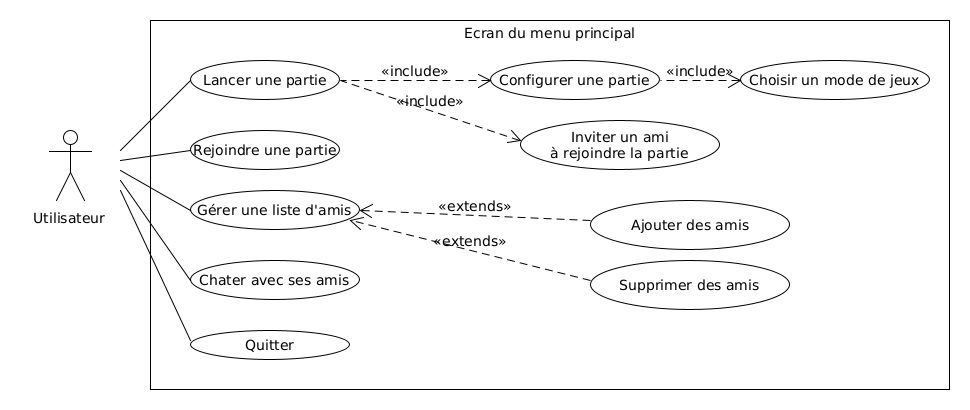
\includegraphics[scale=0.5]{img_fonctionnel/use_case_user_ecran_principal.png}
    \label{fig:user_menu_principal}
    \caption{Menu principal}
\end{figure}

Le menu principal est la première interface que l'utilisateur voit lorsqu'il lance le jeu.
Elle reprend les informations suivantes:
\begin{itemize}
    \item[-] La liste des amis
    \item[-] Les notifications (si l'utilisateur a reçu un message)
    \item[-] Les différents menus accessibles depuis l'écran principal 
\end{itemize}

\subsection{Lancement d'une partie}
Lors du lancement d'une partie le joueur doit simplement fixer les règles en choisissant :
\begin{itemize}
	\item[-] Le type de partie : \textbf{classique} ou \textbf{commandant}
    \item[-] Le type de chrono: \textbf{classique} ou \textbf{pendule}
	\item[-] Le temps d'une partie : au maximum \textbf{15 minutes}
	\item[-] Le temps par tour d'un joueur : au maximum \textbf{30 secondes}
\end{itemize}

Après quoi il sera redirigé vers un lobby, auquel il pourra inviter des joueurs. Le rôle d'un joueur est déterminé par l'ordre d'arrivée dans le lobby. 
Le premier joueur est le joueur principal, le second joueur est le joueur secondaire, et tous les autres joueurs sont des spectateurs.
Un joueur peut aussi rejoindre le lobby sans recevoir d'invitation directement, en entrant le code de la partie.
Si au moins un joueur à rejoint la partie, le joueur principale peut lancer la partie.
Mais avant que la partie ne puisse commencer, il faudra placer tous les bateaux disponibles sur le board, après quoi la partie se lance.

\subsection{Rejoindre une partie}
Afin de rejoindre une partie, l'utilisateur doit simplement entrer un code de partie qu'il aura reçu de la part du joueur principal.
Notons que le code peut être envoyé par le biais du chat, ou tout autre moyen de communication.
Si le joueur joue depuis l'interface graphique, il peut simplement rejoindre la partie en cliquant sur la notification qui apparaitra lorsqu'il recevra le code de partie.


\subsection{Gérer sa liste d'ami}
Chaque utilisateur possède une liste d'amis. Chaque joueur peut ajouter autant d'ami qu'il le souhaite, mais ne peut pas supprimer un ami.
La liste d'ami permet d'initier chat avec l'ami, ce qui permet de notamment communiquer avec lui, mais également de lui envoyer des codes de partie.
Notons que deux joueurs ne doivent pas forcément être amis pour jouer ensemble, il suffit qu'un joueur envoie un code de partie à un autre joueur pour qu'il puisse rejoindre la partie.

\subsection{Chat}
Un joueur peut communiquer avec ses amis via le chat. Si l'utilisateur n'est pas en ligne, il peut tout de même envoyer un message, 
qui sera reçu par l'ami lorsqu'il se connectera.
Le joueur recoit une nouvelle notification lorsqu'il reçoit un message.

\end{document}